\section{Arquitectura de Solución}
Se desarrollará una aplicación la cual contará con módulos móvil y módulos web que, la cual tendrá una arquitectura como se muestra en la Figura \ref{fig:arquitecturaPropuesta}, dicha aplicación ayudará al sector turístico ya que proporcionará información sobre rutas turísticas y áreas de interés de una localidad en particular.

\begin{figure}[htbp]
	\begin{center}
		\hypertarget{fig:arquitecturaPropuesta}{
			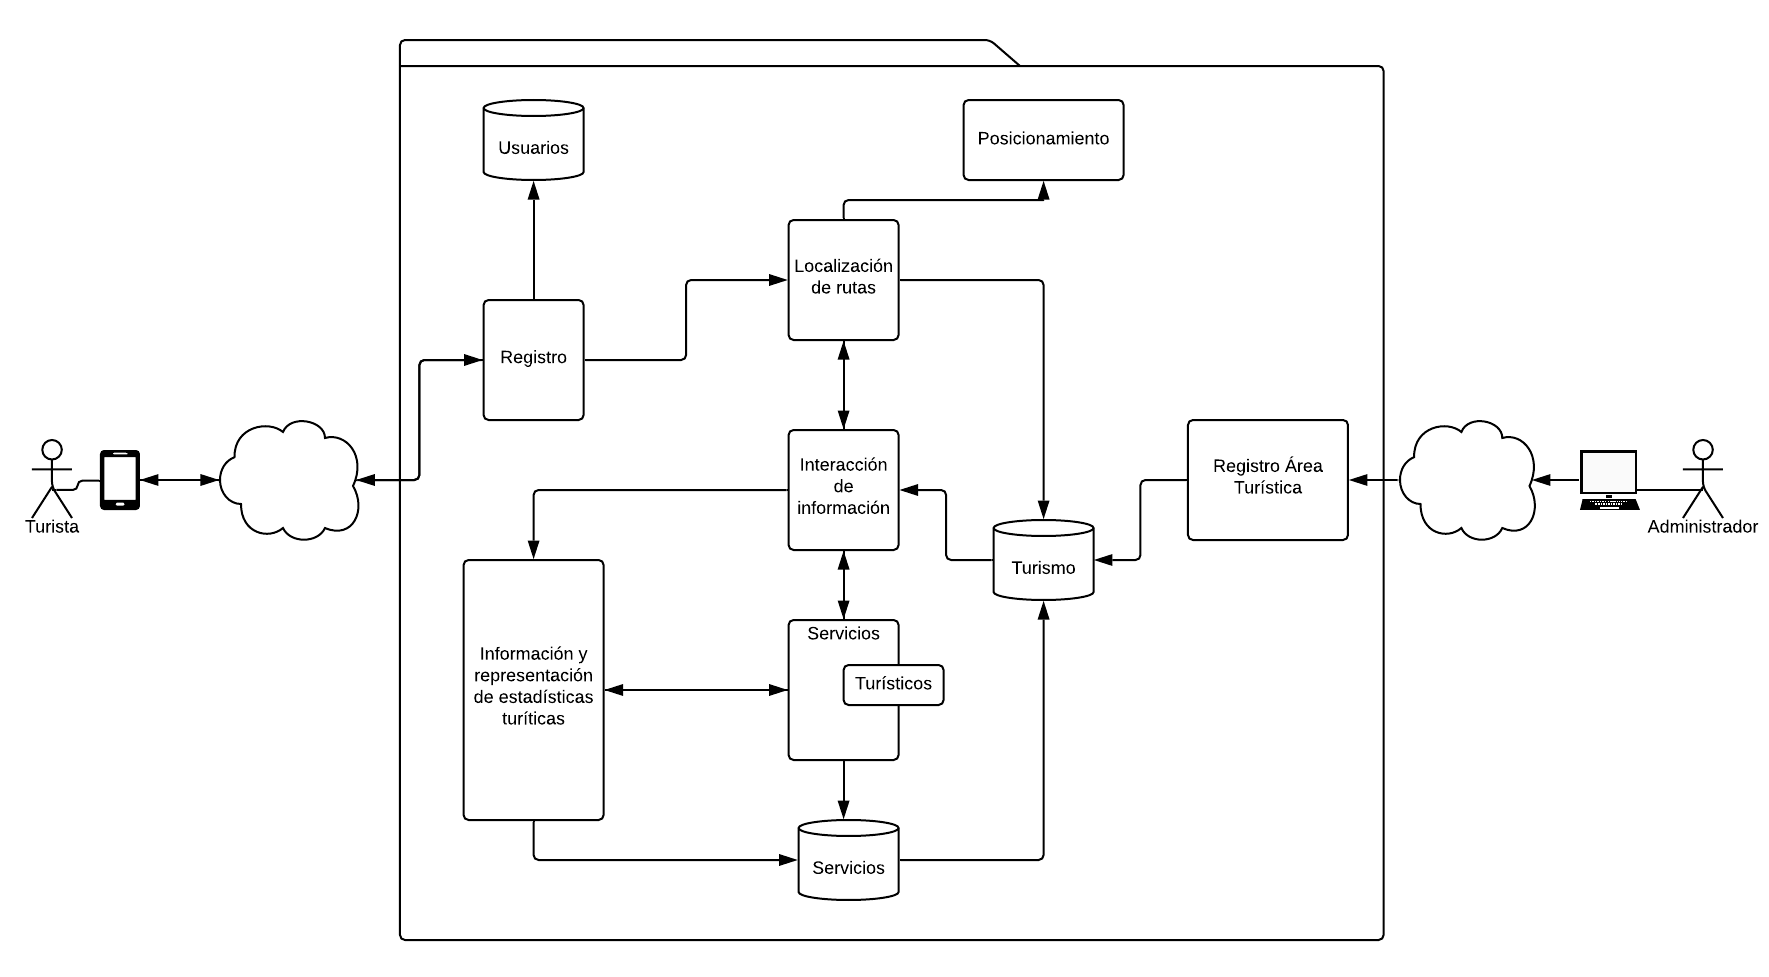
\includegraphics[scale=.4]{propuestaSolicion/turismo/images/arquitecturaPropuesta}
			\caption{Arquitectura de propuesta de solución}
		}
		\label{fig:arquitecturaPropuesta}
	\end{center}
\end{figure}

\newpage
Como puede observarse en la Figura \ref{fig:arquitecturaPropuesta}: \hyperlink{fig:arquitecturaPropuesta}{Arquitectura de propuesta de solución}, la aplicación móvil propuesta para el Trabajo Terminal contará con dos actores: Turista y Administrador.\\

El actor \textbf{Administrador} será el encargado de hacer el registro de las áreas turísticas, esto a través de una aplicación web,  para que posteriormente el actor \textbf{Turista} pueda acceder a esta información mediante la aplicación móvil. \\

El actor \textbf{Turista} tendrá la posibilidad de registrarse en la aplicación para poder contar con el servicio que ésta ofrece, dentro de la aplicación se generarán rutas turísticas basadas en la localización del usuario y de esta forma podrá consultarse los servicios turísticos que se ofrecen dentro del área localizada.\\

Así mismo se contará con un módulo de \textbf{Información y representación de estadísticas turísticas} en el cual se trabajará con la información del usuario para la generación de rutas, sugerencia de sitios y servicios disponibles en la zona localizada.
